\chapter{Multi-Party Computation}

\section{Introduction}
Multi-Party Computation (MPC), also known as Secure Function Evaluation, allows two or more parties
to correctly compute a function of their private inputs without exposure, i.e., without
the input of one party being revealed to the other parties.\\
A generic function \textit{f} receives as input a set $A = \{a_1,a_2,\dots,a_n\}$
of arguments, where $a_i$ is the input of the i-th party, and $1\leq i\leq n$, and outputs a value \textit{z}, which represents the result
of the joint computation of \textit{f}, as shown in Figure \ref{fig:mpcscheme}.\\
The output of \textit{f} is given by the following expression,
\begin{equation}\label{eq:mpc}
z = f(a_1,a_2,\dots,a_n)
\end{equation}

\renewcommand{\figurename}{Figure}
\begin{figure}[H]
\centering
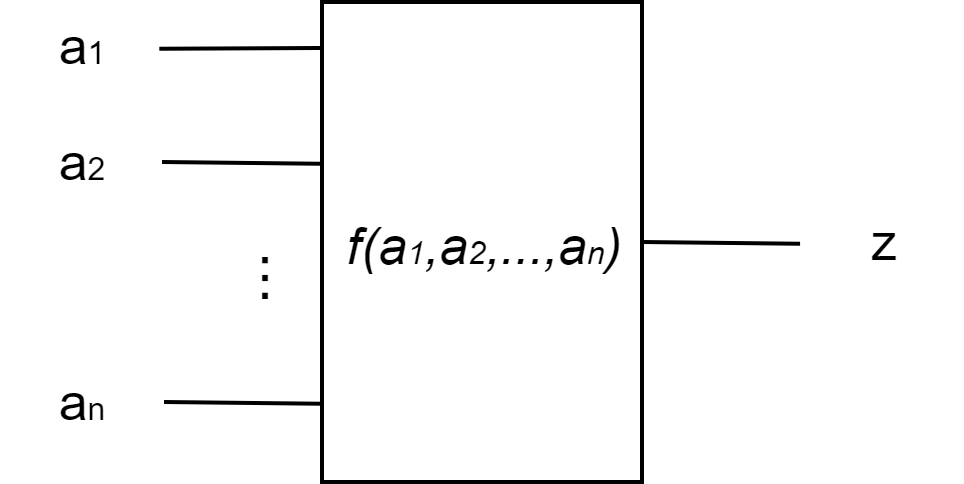
\includegraphics[width=.45\linewidth]{./figures/mpc_scheme}
\caption{Multi-Party Computation Scheme}
\label{fig:mpcscheme}
\end{figure}
\pagebreak

\section{Two-Party Computation}
Two-Party Computation (2PC) is a specific case of MPC, where a generic function \textit{f} receives as input a set $A = \{a,b\}$
of arguments, where \textit{a} is the input from the first party and \textit{b} is the input from the second,
and outputs a value \textit{c}, as shown in Figure \ref{fig:tpcscheme}.\\
The output of \textit{f} is given by the following expression,
\begin{equation}\label{eq:tpc}
c = f(a,b)
\end{equation}

\renewcommand{\figurename}{Figure}
\begin{figure}[H]
\centering
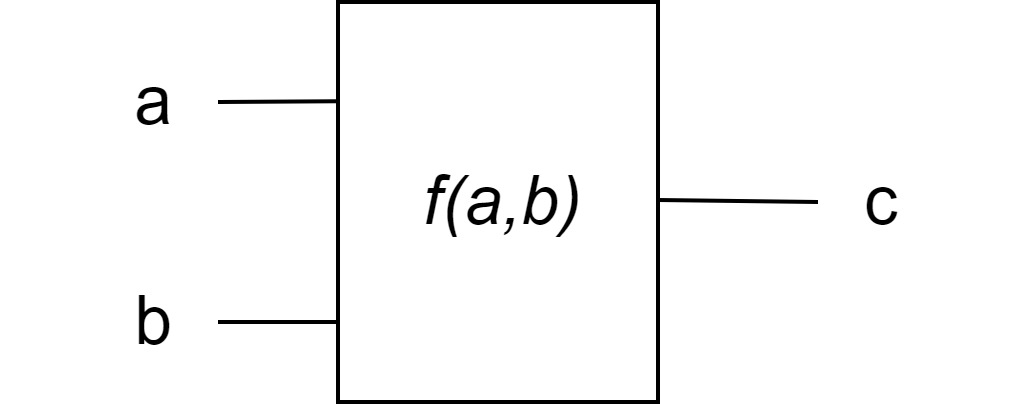
\includegraphics[width=.35\linewidth]{./figures/two_party_computation_scheme}
\caption{Two-Party Computation Scheme}
\label{fig:tpcscheme}
\end{figure}

\section{Garbled Circuit}
In 1986, Andrew Yao proposed the Garbled Circuit protocol (GC), that addresses the specific case
of Two-Party Computation (2PC), without the presence of a trusted third party.\\
GC allows a secure evaluation of a function given
as a Boolean circuit that is represented as a series of logic gates.\\

\bibliography{./chapter/mpcomputation}